\chapter[Aspectos gerais do funcionamento do sistema]{Aspectos gerais do funcionamento do sistema}
u
Inicialmente, todos os módulos do sistema estarão ativados. Através da equação (2) consegue-se inferir a distância mínima que um veículo, trafegando a 120 km/h e que deseja ultrapassar um automóvel de 19,8 m (comprimento máximo de um veículo), trafegando a 60 km/h, deve ter de outro veículo com 120 km/h vindo na direção contrária, de modo que saia de sua faixa com, pelo menos 5 m de distância do carro a ser ultrapassado e volte para a faixa com, pelo menos 5 m de distância do mesmo carro.

\begin{figure}[h]
  \centering
  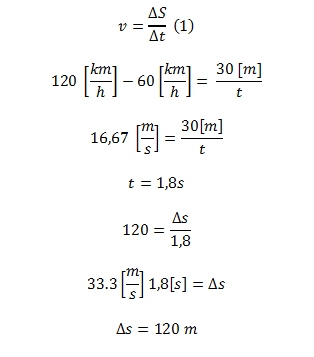
\includegraphics[width=150px, scale=1]{figuras/formula_func}
  \caption{Equação 2}
\end{figure}

O microprocessador estará monitorando qualquer sinal de intenção de ultrapassagem, serão utilizados três parâmetros para definir essa intenção, o uso da seta, a diminuição da distância do carro que quer realizar a ultrapassagem para o carro da frente, identificado pela câmera, radar e lidar, a rotação do volante, identificado pelo sensor de rotação e a mudança de faixa, identificada pela câmera. Tendo identificado a intenção do motorista, o microprocessador enviará sinal para que os dispositivos coletem mais informações de velocidade e posição, após a coleta de dados, que será enviado ao microprocessador, será feito os cálculos e definido se há viabilidade para ultrapassar. A seguir, será descrito o funcionamento do sistema e a integração dos dispositivos.

A figura abaixo juntamente com o quadro explicativo, ilustram melhor esse funcionamento.

\begin{figure}[h]
  \centering
  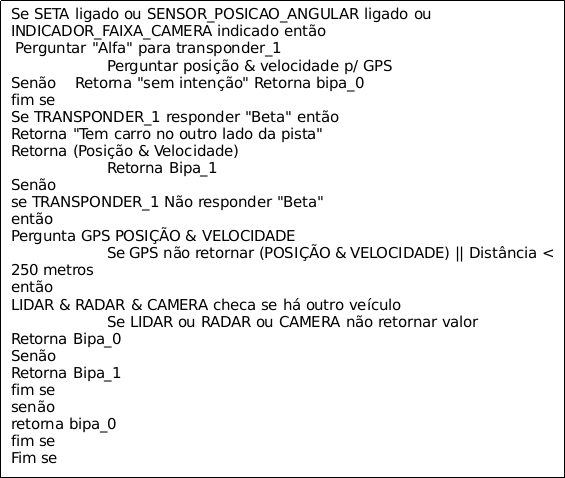
\includegraphics[width=250px, scale=1]{figuras/quadro_explicativo}
  \caption{Quadro Explicativo do Algoritmo Básico do Funcionamento do CIAC}
\end{figure}

\begin{figure}[h]
  \centering
  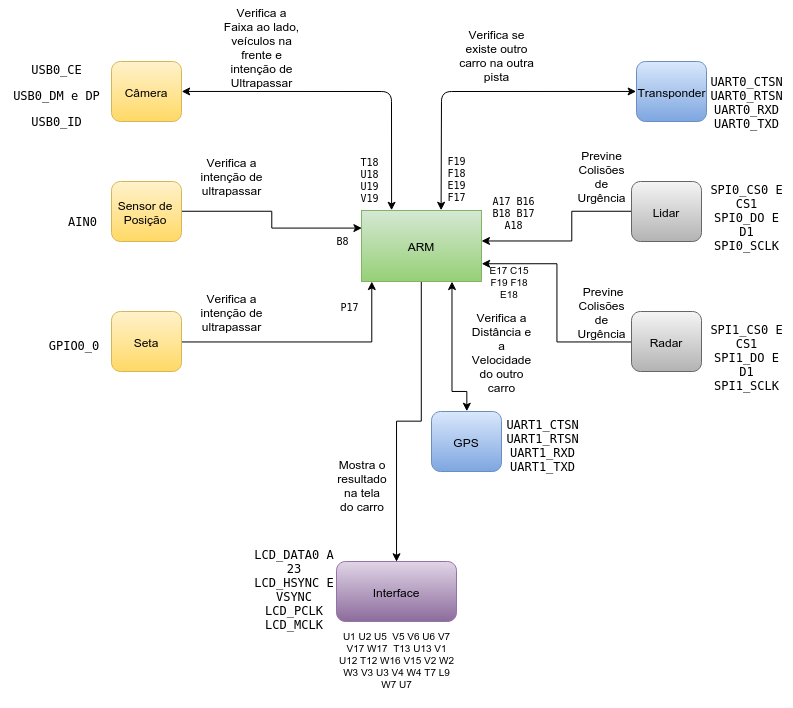
\includegraphics[width=250px, scale=1]{figuras/fluxo}
  \caption{Diagrama de funcionamento do CIAC, com esquemático de conexões no microprocessador}
\end{figure}